\chapter{Appendix B} 
\label{appendix:anexo2}

The purpose of this appendix is to explain in more detail how the algorithm works used in SFALib described in sub chapter \ref{sub:sfa_library}.

\begin{enumerate}


\item The algorithm starts by creating an histogram with the vessel velocity data as the one in Figure \ref{fig:app_b_1}. 

\begin{figure}[H]
    \centering
    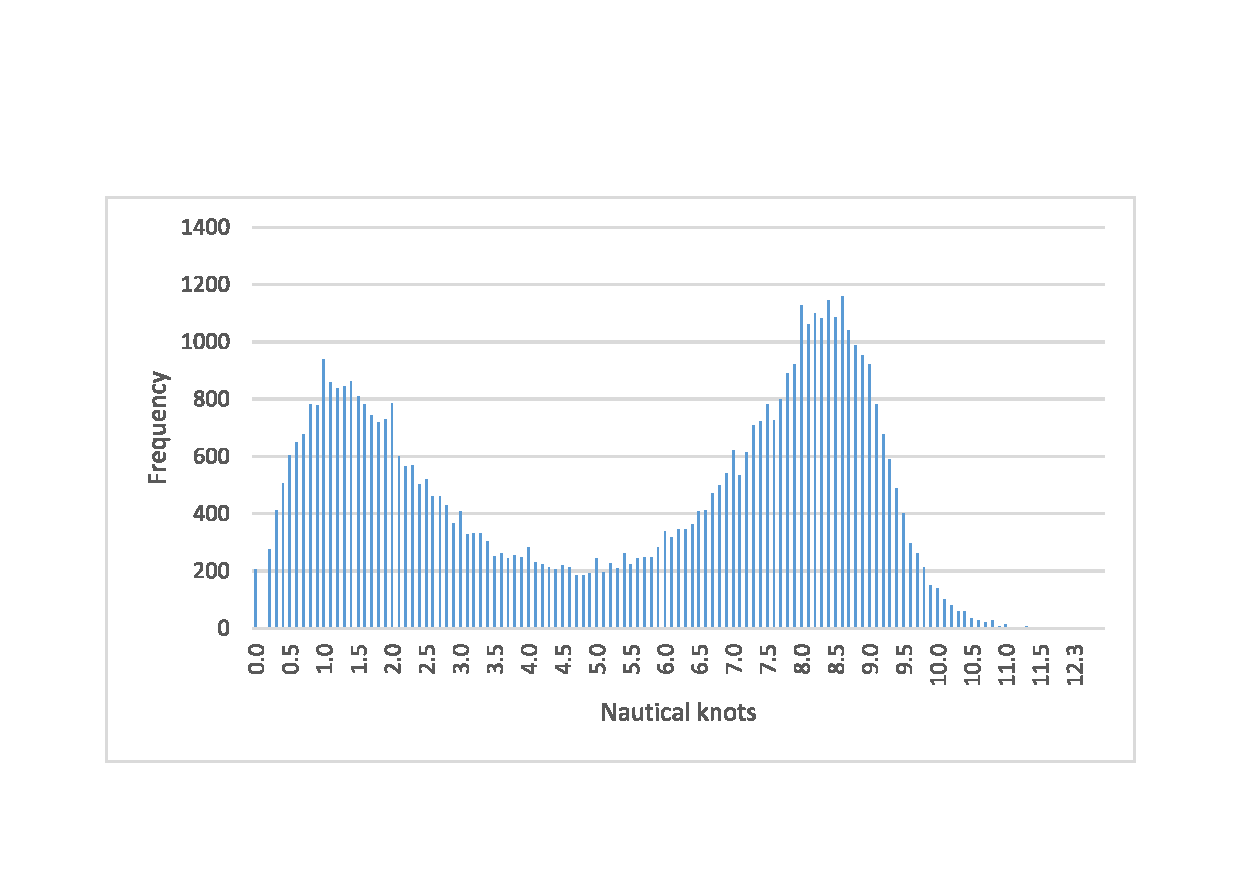
\includegraphics[trim=0 80 0 80,height=0.45\linewidth]{Chapters/img/hist_vessel2.pdf}
    \caption{Create histogram}
    \label{fig:app_b_1}
\end{figure}

\newpage
\item Then remove from the histogram the frequency of value 0.
\begin{figure}[H]
    \centering
    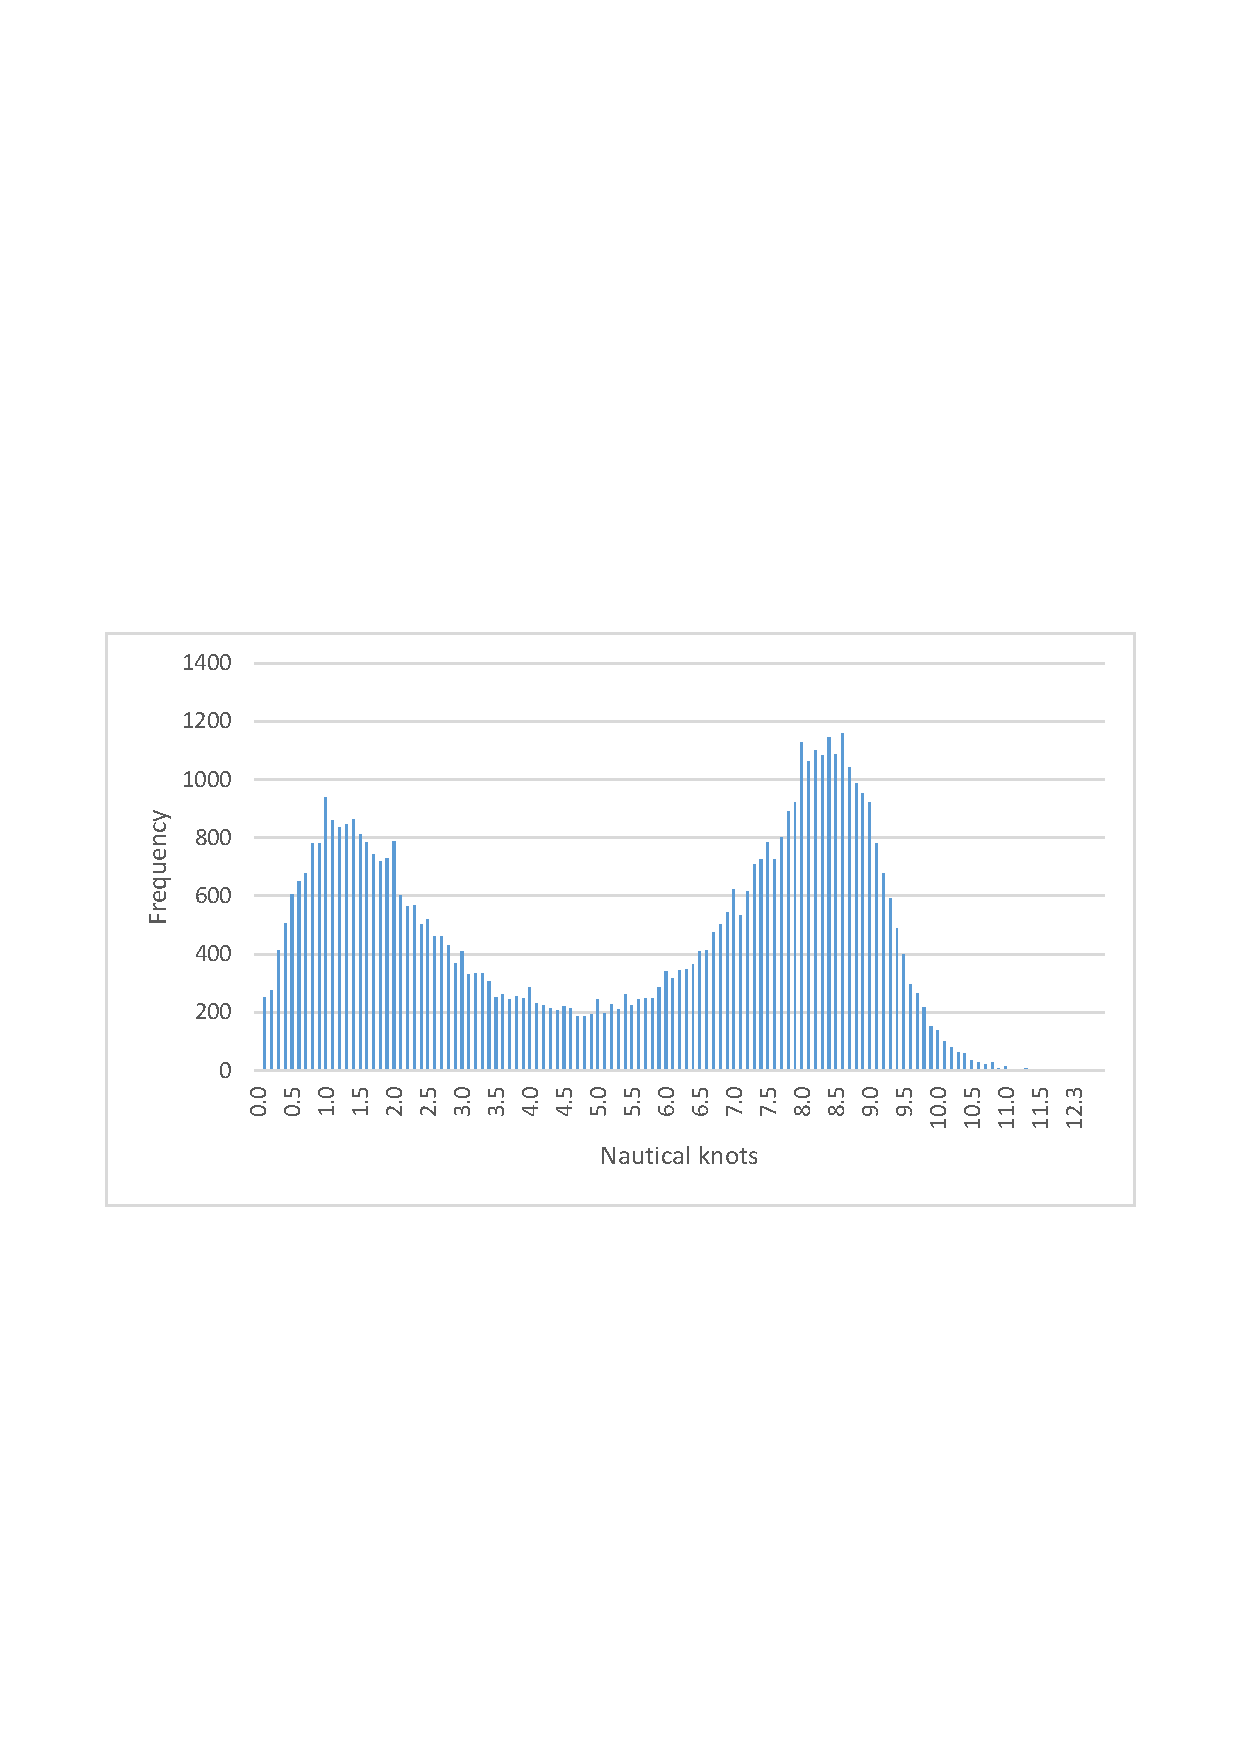
\includegraphics[trim=250 275 250 300,height=0.5\linewidth]{Chapters/img/hc_2.pdf}
    \caption{Remove requency of value 0}
    \label{fig:app_b_2}
\end{figure}

\item Use Hill-Climbing function to get maximum frequency for the velocity of fishing activity.
\begin{figure}[H]
    \centering
    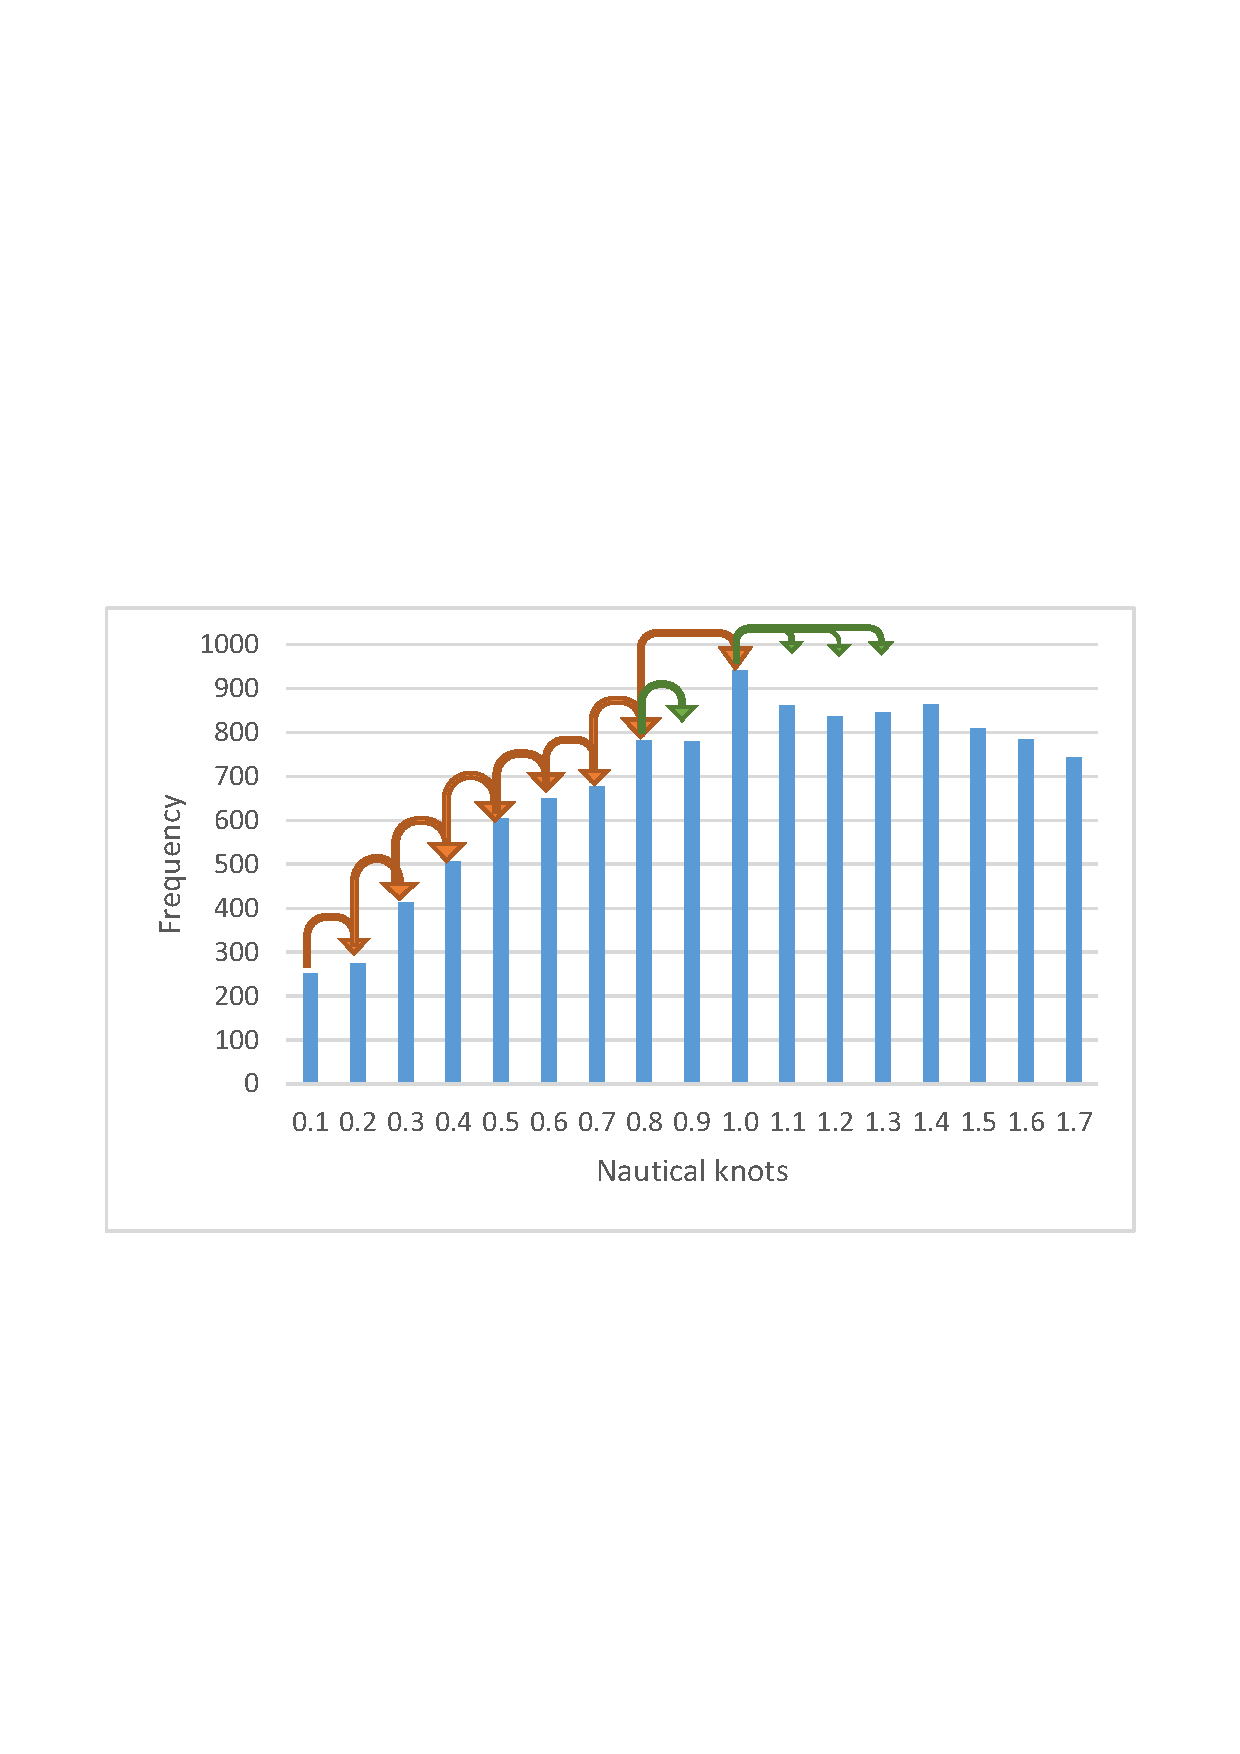
\includegraphics[trim=300 250 300 300,height=0.5\linewidth]{Chapters/img/hc_3.pdf}
    \caption{Find maximum}
    \label{fig:app_b_3}
\end{figure}
\newpage
\item After finding the maximum frequency Hill-Climbing find the next minimum frequency to represent the maximum velocity value of the fishing activity.
\begin{figure}[H]
    \centering
    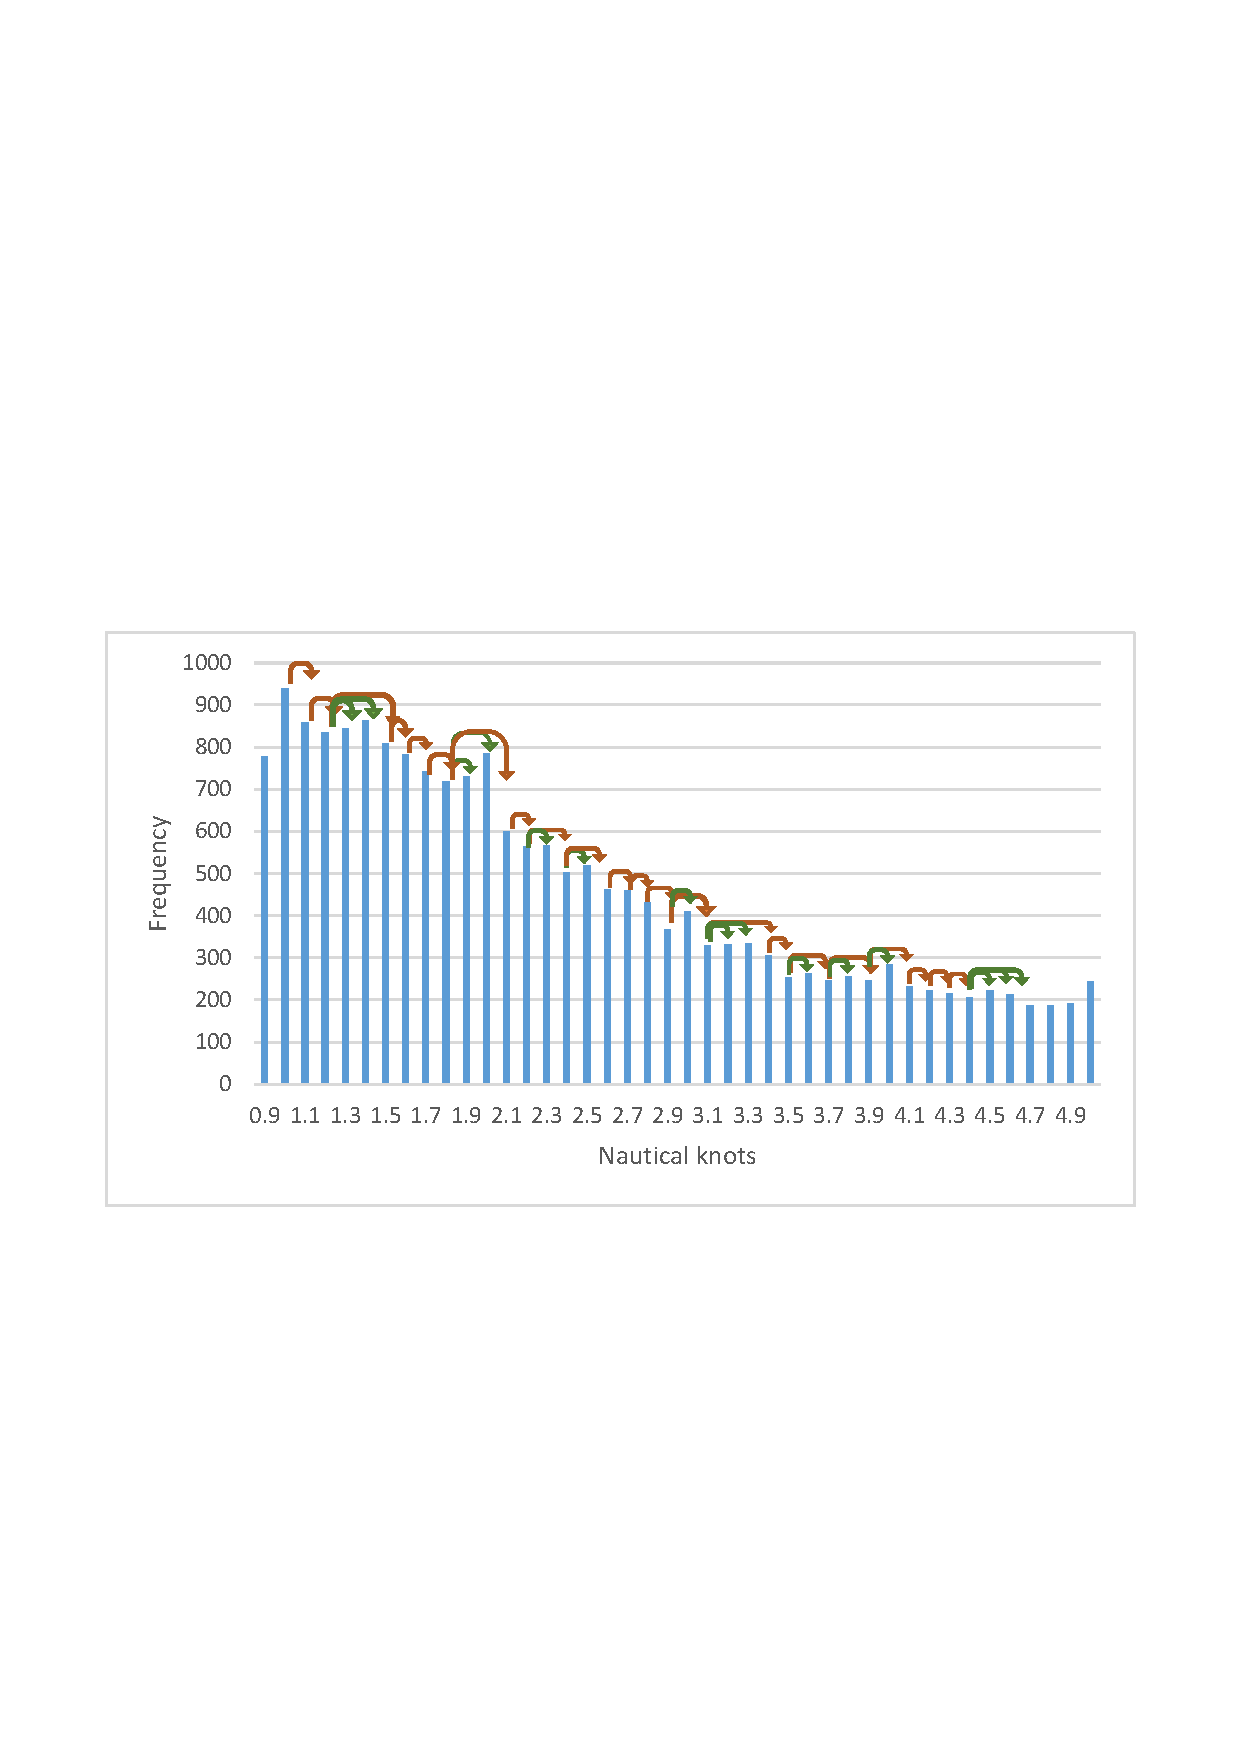
\includegraphics[trim=250 250 250 300,height=0.5\linewidth]{Chapters/img/hc_4.pdf}
    \caption{Find minimum}
    \label{fig:app_b_4}
\end{figure}

\item Remove values greater that the maximum velocity value found in the last step.
\begin{figure}[H]
    \centering
    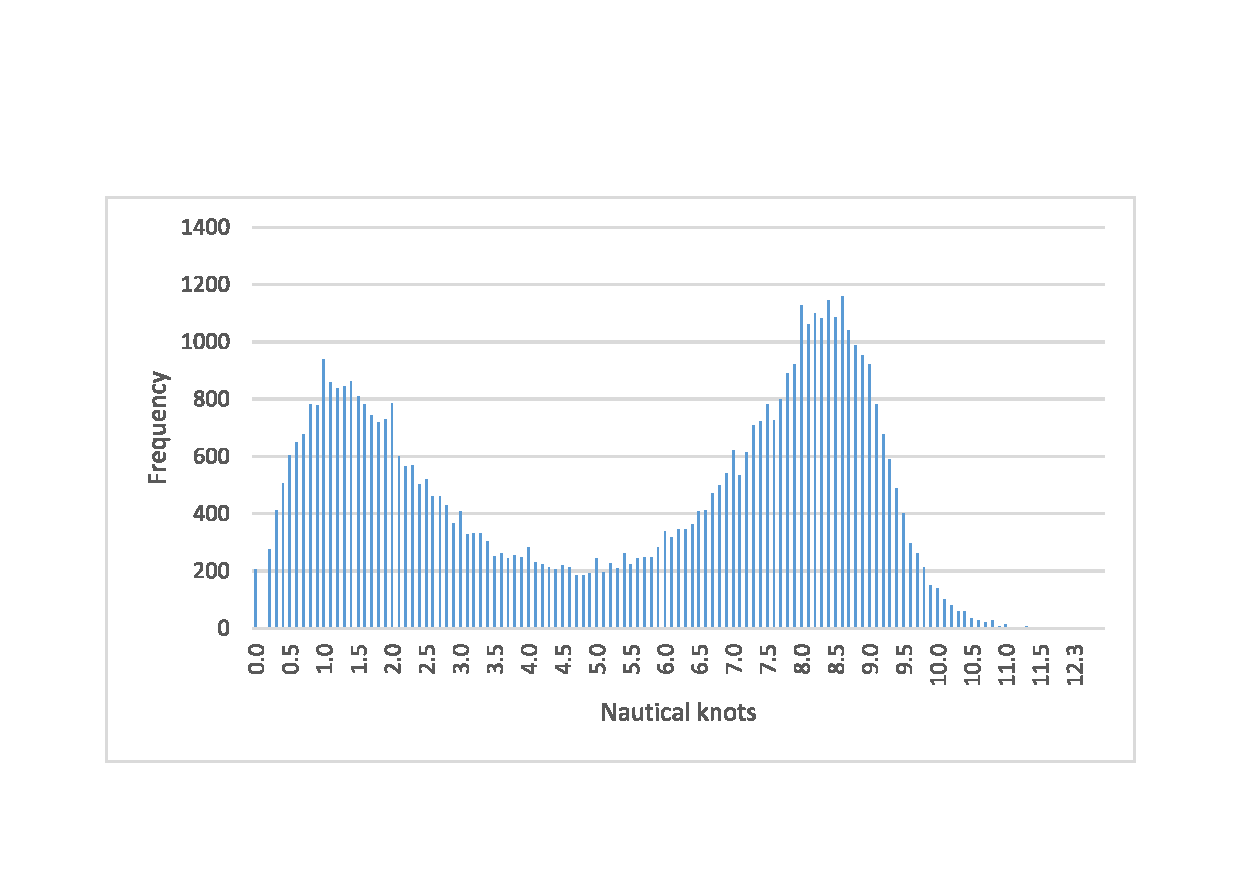
\includegraphics[trim=0 80 0 80,height=0.45\linewidth]{Chapters/img/hist_vessel2.pdf}
    \caption{Remove verge values}
    \label{fig:app_b_5}
\end{figure}
	
%\item Remove values with frequency under 10\%(configurable) of the frequency %found in step 3.

\newpage
\item Calculate Kernel Density distribution.
\begin{figure}[H]
    \centering
    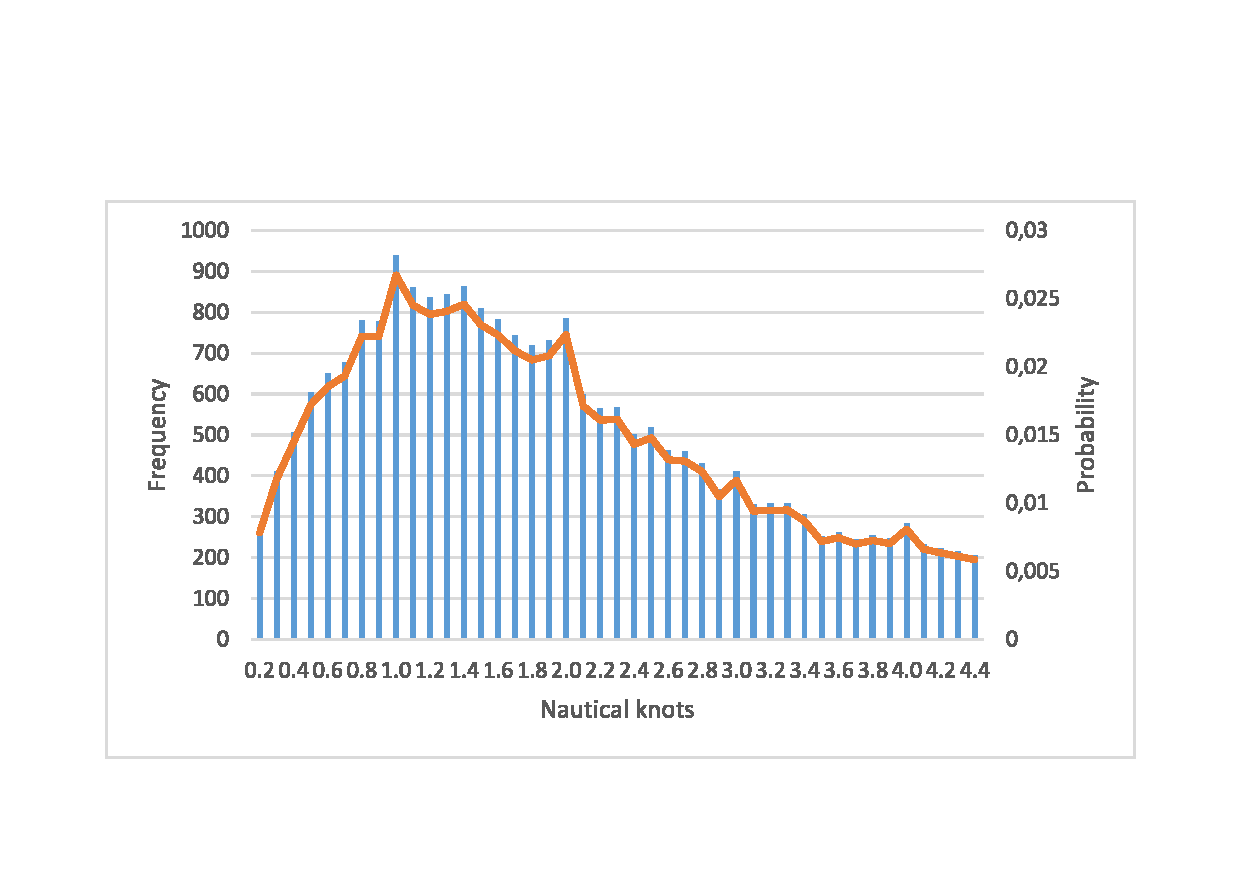
\includegraphics[trim=0 80 0 80,height=0.45\linewidth]{Chapters/img/hist_kernel.pdf}
    \caption{Kernel Density distribution}
    \label{fig:app_b_6}
\end{figure}

\item Calculate cumulative function of Kernel density distribution.
\begin{figure}[H]
    \centering
    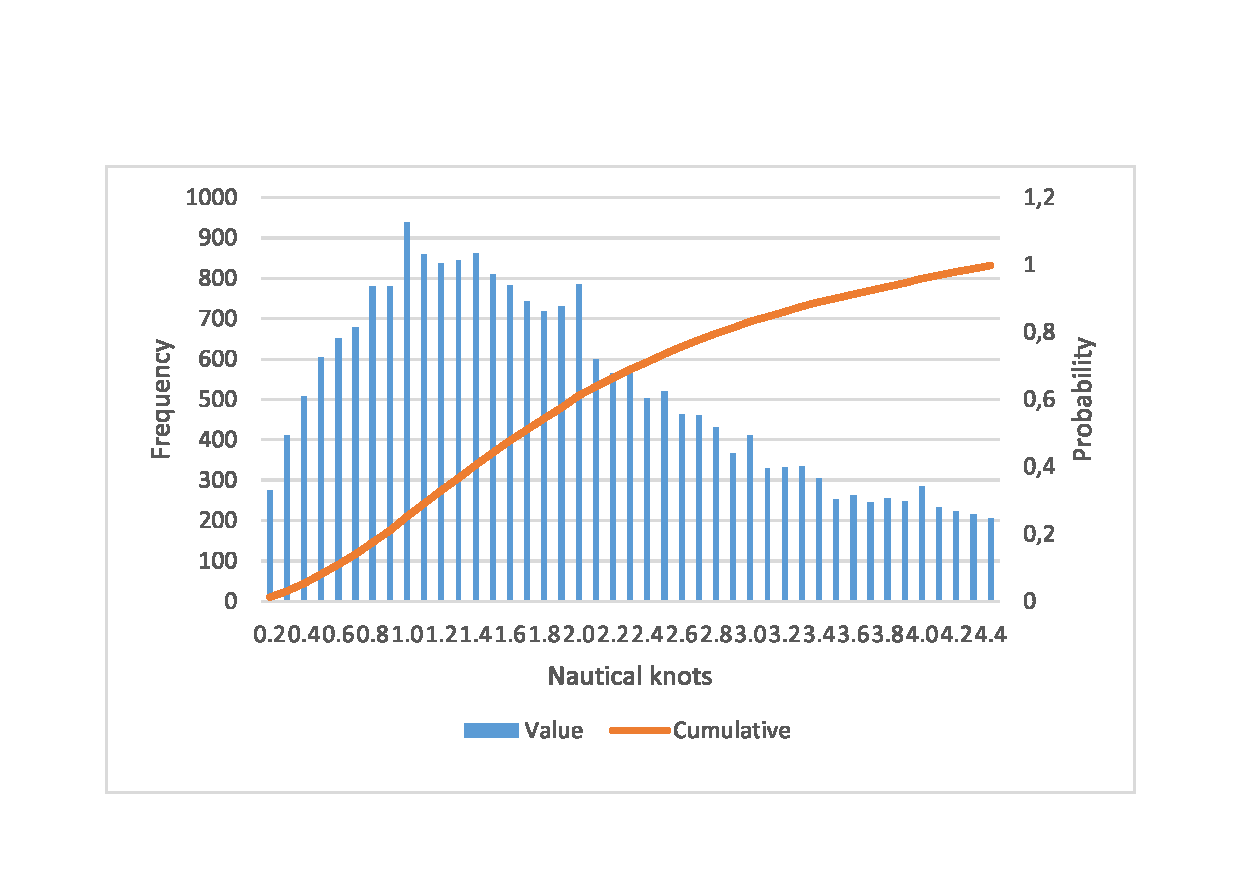
\includegraphics[trim=0 80 0 80,height=0.45\linewidth]{Chapters/img/hist_comulative.pdf}
    \caption{Cumulative Kernel Density}
    \label{fig:app_b_7}
\end{figure}
\newpage % trim={<left> <lower> <right> <upper>}
\item Set margin (configurable, exemple 20\%) of the cumulative function and get fishing velocity limits of the vessel.
\begin{figure}[H]
    \centering
    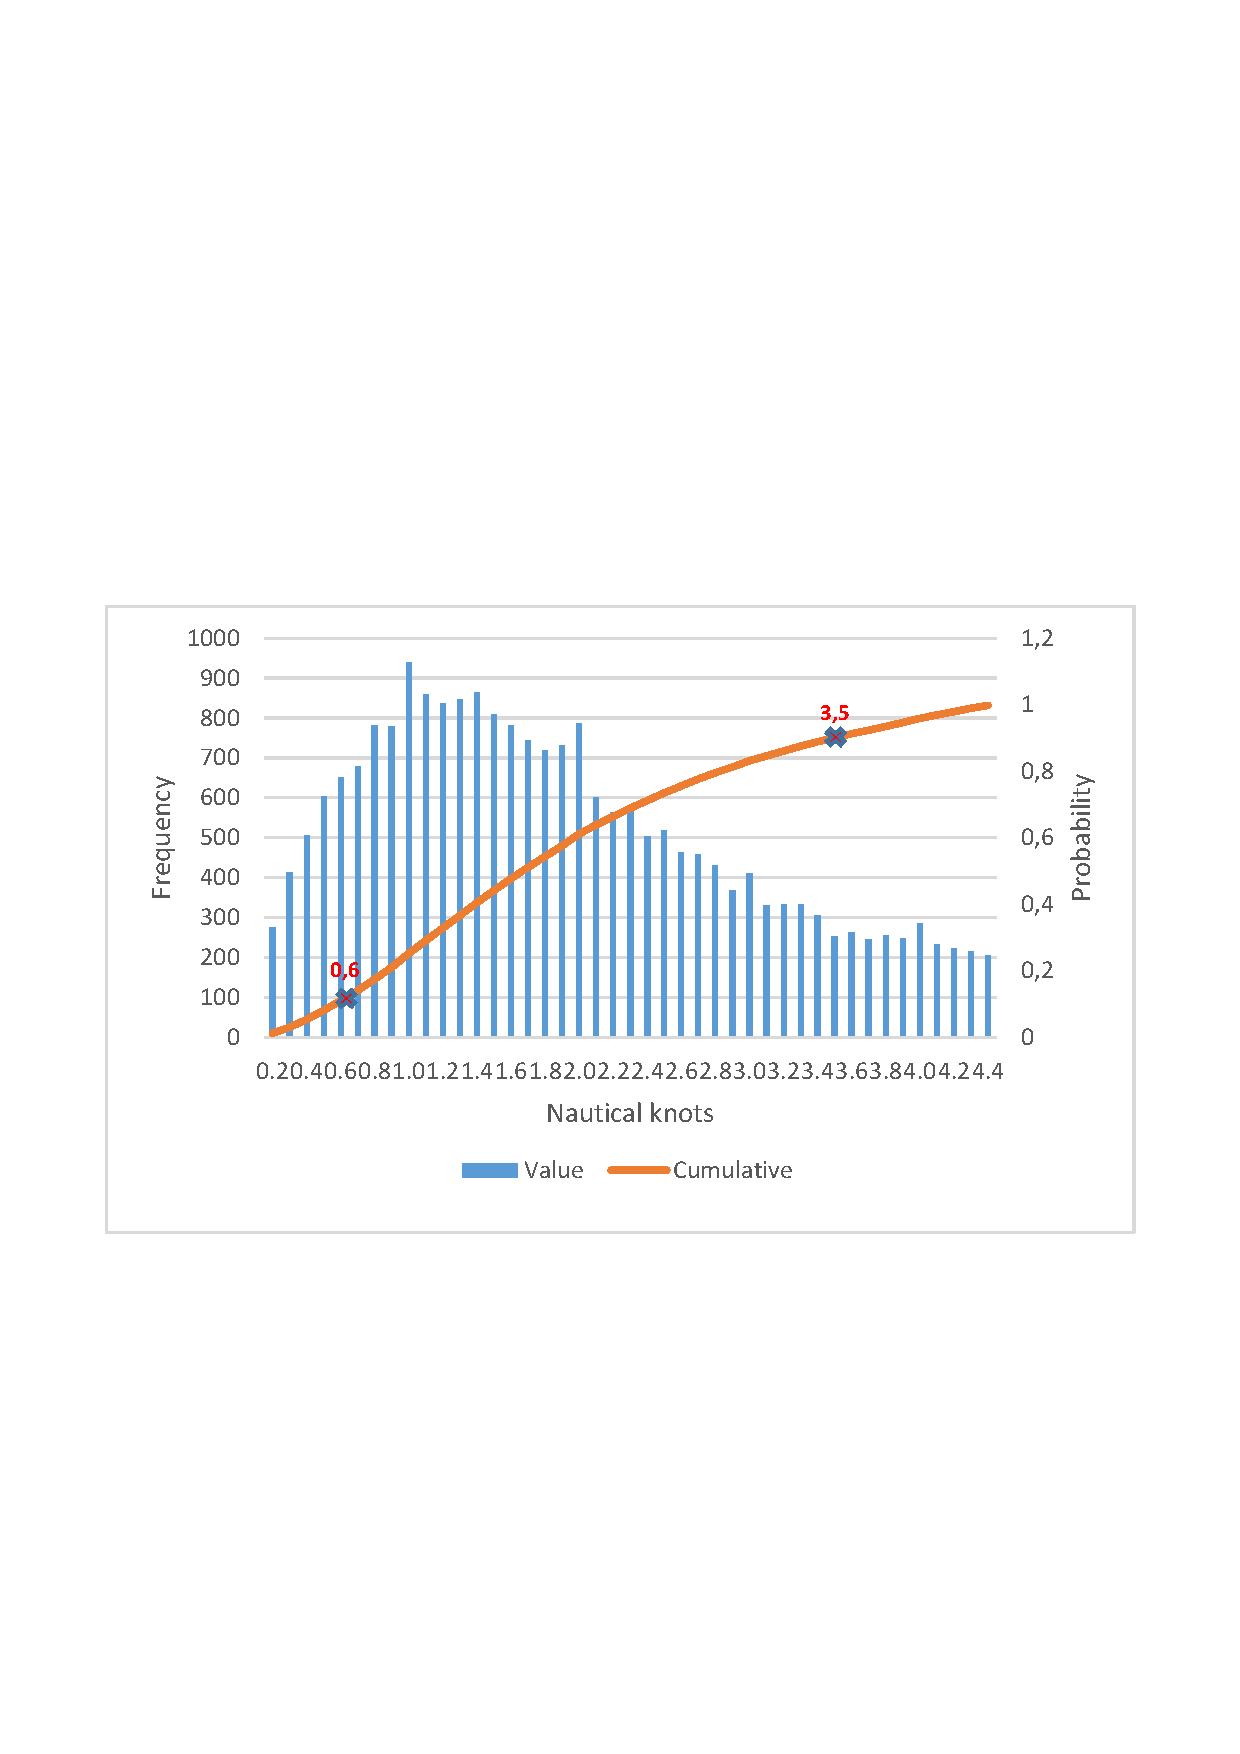
\includegraphics[trim=300 250 300 300,height=0.5\linewidth]{Chapters/img/hc_8.pdf}
    \caption{Set margin and get limits}
    \label{fig:app_b_8}
\end{figure}


\end{enumerate}

%\begin{figure}[H]
%    \centering
%    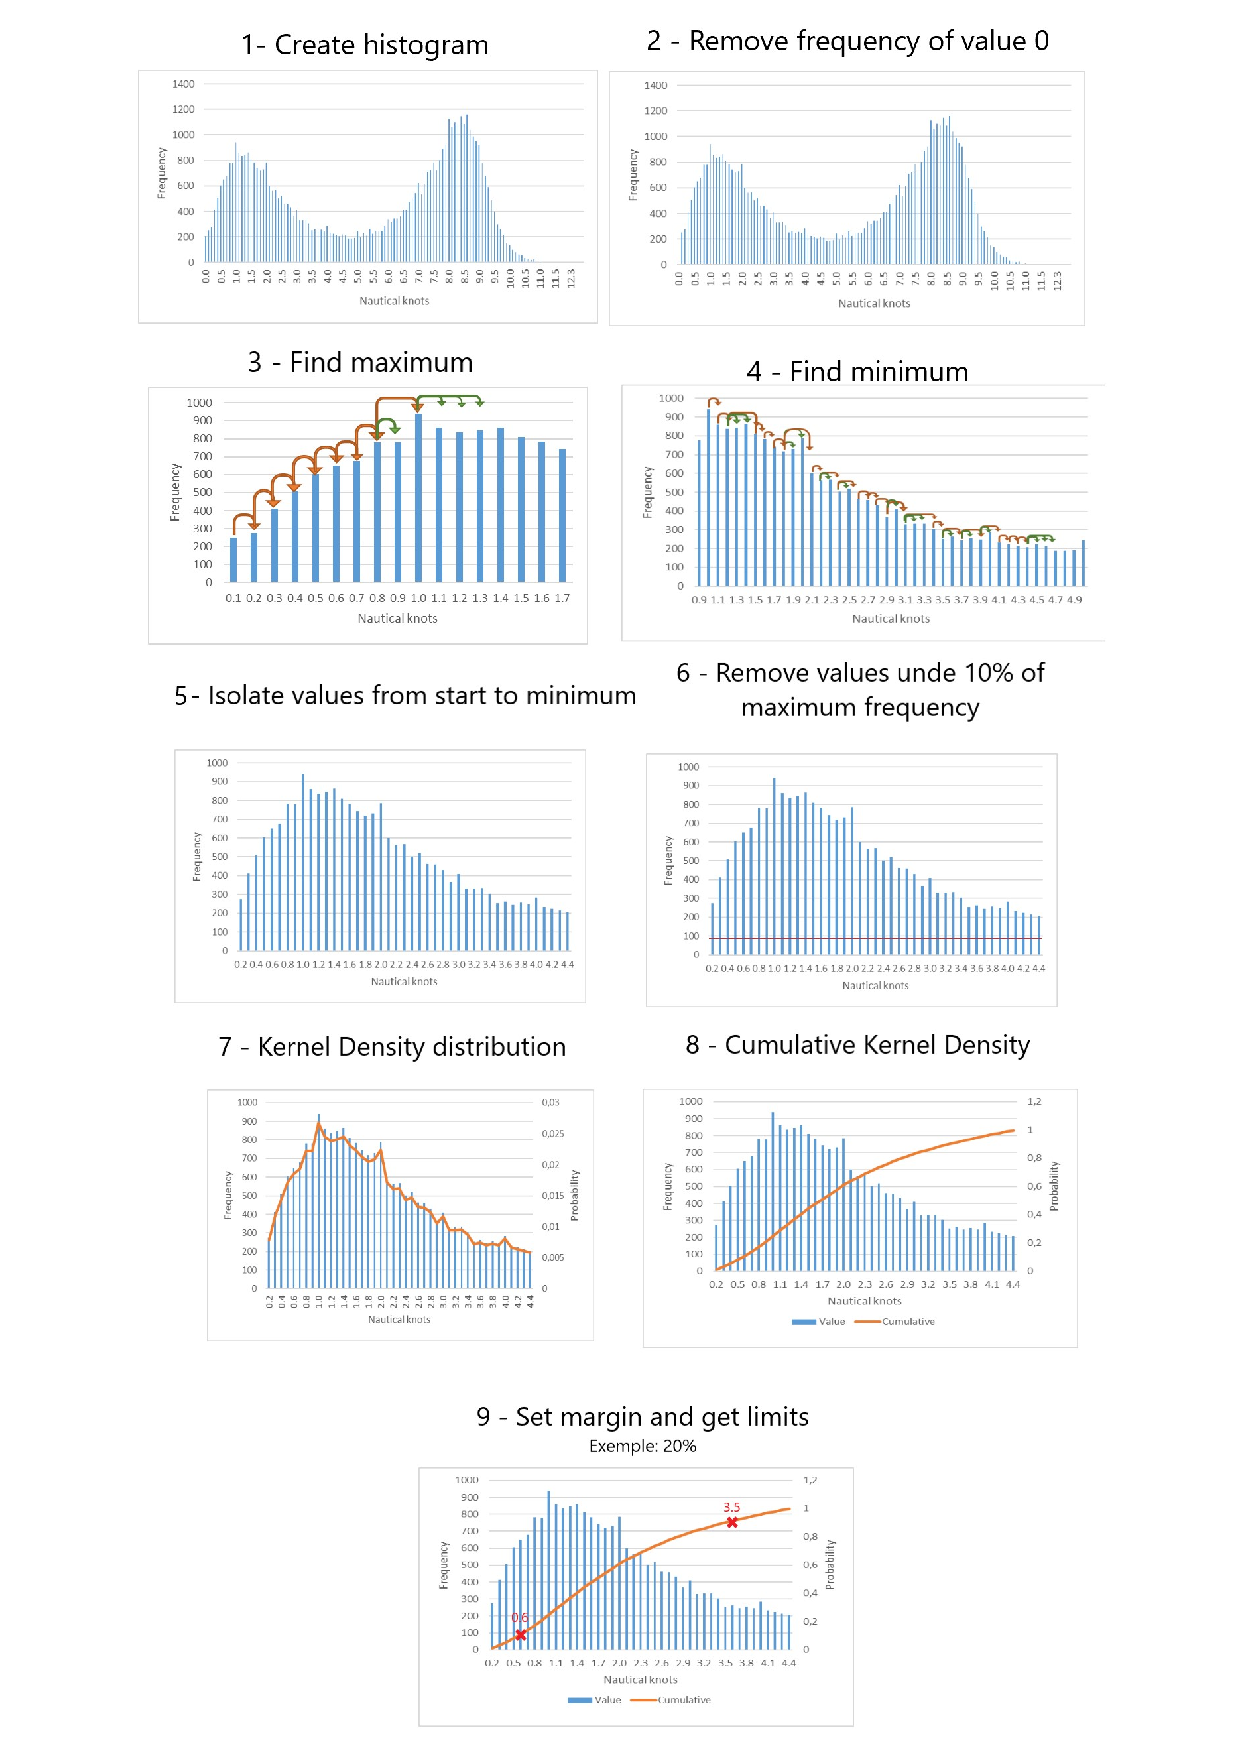
\includegraphics[trim=0 0 0 0,height=0.9\linewidth]{Chapters/img/hc.pdf}
%    \caption{XXXXX}
%    \label{fig:hist_comulative}
%\end{figure}

